% !TEX encoding = UTF-8 Unicode
% !TEX TS-program = xelatex

\chapter{二次曲線}

\section{拋物線}

\begin{tikzpicture}
\coordinate (cAPt) at (0,0);
\coordinate (caxisUP) at (0,3.5);
\coordinate (caxisDOWN) at (0,-0.5);
\coordinate (cPPt) at (-3,3);
\coordinate (cQPt) at (3,3);
\coordinate (cRPt) at (-4,2);
\coordinate (cSPt) at (4,2);

\draw[draw=black, every edge/.append style={draw=black, dashed}] (caxisUP) edge (caxisDOWN);
\draw[name path=PAR1] (cAPt) parabola (cPPt);
\draw[name path=PAR2] (cAPt) parabola (cQPt);

\draw[name path=LINE1] (cRPt) -- (cSPt); 

\path [name intersections={of=PAR1 and LINE1,by=cCPt}];

\path [name intersections={of=PAR2 and LINE1,by=cDPt}];

\draw[ultra thick,fill] (cCPt) circle (1pt);
\draw[ultra thick,fill] (cDPt) circle (1pt); 
\draw[ultra thick,fill] (cDPt) circle (1pt); 


\coordinate (cMPt) at  ($ (cCPt) !0.5! (cDPt) $);
\draw (cCPt) -- node[sloped] {$\parallel$} (cMPt);

\draw (cMPt) -- node[sloped] {$\parallel$} (cDPt);

\node[below] at (caxisDOWN){$x=4$};
\node[below left] at (cCPt){$(1,24)$};
\node[below right ] at (cDPt){$(7,24)$};
\end{tikzpicture}

\begin{tikzpicture}

\begin{scope}
\draw[line width=1.75pt, domain={-2.3}:{2.3}, samples=500] plot[smooth]({\x*\x},\x );

\draw[{{Stealth[scale=1.3,angle'=45]}-{Stealth[scale=1.3,angle'=45]}}, name path=LINE1] (4,2) -- (4,-2) node [ midway, right]{ $3cm$}; ; 

\draw[{{Stealth[scale=1.3,angle'=45]}-{Stealth[scale=1.3,angle'=45]}}, name path=LINE2] (0,-2.3) -- (4,-2.3) node [ midway, below]{ $2cm$};
\node at ( 2 , 0) {甲拋物面鏡}; 
\end{scope}

\begin{scope}[shift={(7,0)}]
\draw[line width=1.75pt, domain={-2.3}:{2.3}, samples=500] plot[smooth]({\x*\x},\x );

\draw[{{Stealth[scale=1.3,angle'=45]}-{Stealth[scale=1.3,angle'=45]}}, name path=LINE1] (4,2) -> (4,-2) node [ midway, right]{ $3cm$}; ; 

\draw[{{Stealth[scale=1.3,angle'=45]}-{Stealth[scale=1.3,angle'=45]}}, name path=LINE2] (0,-2.3) -- (4,-2.3) node [ midway, below]{ $3cm$}; 
\node at ( 2 , 0) {乙拋物面鏡}; 

\end{scope}

\end{tikzpicture}

\pgfmathdeclarefunction{myfuncta}{1}{%
    \pgfmathparse{-1*(#1)^(0.5)}%
}
\pgfmathdeclarefunction{myfunctb}{1}{%
    \pgfmathparse{1*(#1)^(0.5)}%
}
\begin{tikzpicture}
%\pgfplotsset{ticks=none}
\begin{axis}[
unit vector ratio*=1 1 1,
axis lines = middle,
axis line style = {-{Stealth[scale=1.3,angle'=45]}},
hide y axis,
hide x axis,
width=7cm,
xlabel={$x$},
ylabel={$y$},
xtick={},
ytick={},
ymax =2.5,
ymin =-4.5,
xmax = 3.5,
xmin = -2.5
]
%Below the red parabola is defined
\addplot[samples=300,domain=0:3] {myfuncta(x)};
\addplot[samples=300,domain=0:3] {myfunctb(x)};
\addplot[samples=300,domain=0:2, {-{Stealth[scale=1.3,angle'=45]}}] {-2};
\addplot[samples=300,domain=2:0, {-{Stealth[scale=1.3,angle'=45]}}] {-2};
%\addlegendentry{$\$}
%Here the blue parabloa is defined

\end{axis}
\end{tikzpicture}

\begin{tikzpicture}
\coordinate (cAPt) at (0,0);
\coordinate (caxisUP) at (0,3.5);
\coordinate (caxisDOWN) at (0,-0.5);
\coordinate (cPPt) at (-3,3);
\coordinate (cQPt) at (3,3);
\coordinate (cRPt) at (-4,2);
\coordinate (cSPt) at (4,2);

\draw[draw=black, every edge/.append style={draw=black, dashed}] (caxisUP) edge (caxisDOWN);
\draw[name path=PAR1] (cAPt) parabola (cPPt);
\draw[name path=PAR2] (cAPt) parabola (cQPt);

\draw[name path=LINE1] (cRPt) -- (cSPt); 

\path [name intersections={of=PAR1 and LINE1,by=cCPt}];

\path [name intersections={of=PAR2 and LINE1,by=cDPt}];

\draw[ultra thick,fill] (cCPt) circle (1pt);
\draw[ultra thick,fill] (cDPt) circle (1pt); 
\draw[ultra thick,fill] (cDPt) circle (1pt); 


\coordinate (cMPt) at  ($ (cCPt) !0.5! (cDPt) $);
\draw (cCPt) -- node[sloped] {$\parallel$} (cMPt);

\draw (cMPt) -- node[sloped] {$\parallel$} (cDPt);

\node[below] at (caxisDOWN){$x=4$};
\node[below left] at (cCPt){$(1,24)$};
\node[below right ] at (cDPt){$(7,24)$};
\end{tikzpicture}

\section{橢圓}

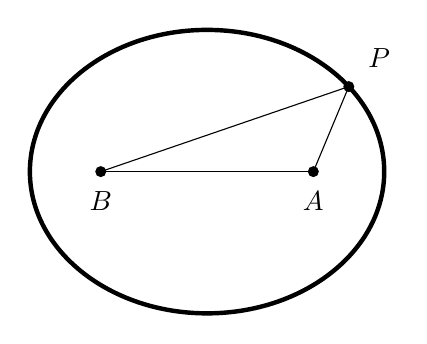
\begin{tikzpicture}[scale=0.45]


\coordinate (cF1Pt) at (3, 0);
\coordinate (cF2Pt) at (-3, 0);
\coordinate (cP) at (4, 2.4);
\draw [ultra thick](0,0) ellipse (5 and 4);

\draw (cF1Pt) -- (cF2Pt) ;
\draw (cP) -- (cF2Pt) ;
\draw (cF1Pt) -- (cP) ;


\foreach \v/\u/\t in 
{cF1Pt/270/$A$,
    cF2Pt/270/$B$,
    cP/45/$P$
}
{
    \draw[ultra thick,fill] (\v) circle (2.5pt);
    \node[label=\u:\t] at (\v){};
};

\end{tikzpicture}

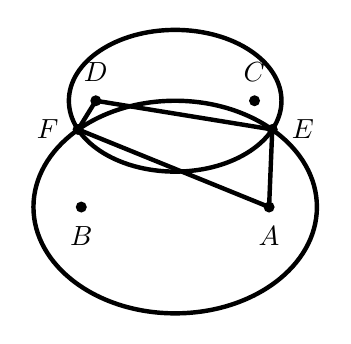
\begin{tikzpicture}[scale=0.45]
\coordinate (cAPt) at (2.65, 0);
\coordinate (cBPt) at (-2.65, 0);
\coordinate (cCPt) at (2.24, 3);
\coordinate (cDPt) at (-2.24, 3);
\coordinate (cEPt) at (2.74,2.19);
\coordinate (cFPt) at (-2.74,2.19);

\draw [ultra thick](0,0) ellipse (4 and 3) ;
\draw [ultra thick](0,3) ellipse (3 and 2);
%\path [name intersections={of=PAR1 and LINE1,by=cCPt}];

\draw [ultra thick](cAPt) -- (cEPt) -- (cDPt) -- (cFPt) -- cycle ;


\foreach \v/\u/\t in 
{   cAPt/270/$A$,
    cBPt/270/$B$,
    cCPt/90/$C$,
    cDPt/90/$D$,
    cEPt/0/$E$,
    cFPt/180/$F$
}
{
    \draw[ultra thick,fill] (\v) circle (2.5pt);
    \node[label=\u:\t] at (\v){};
};
\end{tikzpicture}

\begin{tikzpicture}[scale=1]
\coordinate (cVPt) at (0,0);
\coordinate (cFPt) at (1,0);
\draw[thick, -{Stealth[scale=1.3,angle'=30]}] (-0.2,0) -- (5.2,0) node[below] {$x$};
\draw[thick, -{Stealth[scale=1.3,angle'=30]}] (0,-4.3) -- (0,4.3) node[above] {$y$};

\draw[thick, color=black, domain=0:3.5] plot (\x,{(4*\x)^(1/2)});
\draw[thick, color=black, domain=0:3.5] plot (\x,{-(4*\x)^(1/2)});

\draw [ultra thick]({13/8},0) ellipse ({13/8} and {3/2}) ;

\foreach \v/\u/\t in 
{   cVPt/225/$V$,
    cFPt/310/$F$
}
{
    \draw[ultra thick,fill] (\v) circle (1pt);
    \node[label=\u:\t] at (\v){};
};
\end{tikzpicture}


\begin{tikzpicture}[scale=1]
\coordinate (cAPt) at (4,0);
\coordinate (cDPt) at (-3,{7/4});
\coordinate (cCPt) at (-3,{-7/4});
\coordinate (cOPt) at (0,0);
\coordinate (cFPt) at (-3,0);


\draw[thick, -{Stealth[scale=1.3,angle'=30]}] (-5,0) -- (5,0) node[below] {$x$};
\draw[thick, -{Stealth[scale=1.3,angle'=30]}] (0,-3.5) -- (0,3.5) node[above] {$y$};

\draw [ultra thick](0,0) ellipse ({4} and {sqrt(7)}) ;

\tkzMarkRightAngle[size=0.3](cOPt,cFPt,cDPt)

\foreach \v/\u/\t in 
{   cAPt/315/$A$,
    cDPt/90/$D$
}
{
    \draw[ultra thick,fill] (\v) circle (1pt);
    \node[label=\u:\t] at (\v){};
};

\draw [ultra thick](cAPt) -- (cDPt) -- (cCPt) ;

\end{tikzpicture}

\section{雙曲線}
\section{綜合}

